\chapter{Classification}

\begin{description}
    \item[(Supervised) classification] \marginnote{Classification} 
        Given a finite set of classes $C$ and a dataset $\matr{X}$ of $N$ individuals, 
        each associated to a class $y(\vec{x}) \in C$,
        we want to learn a model $\mathcal{M}$ able to 
        guess the value of $y(\bar{\vec{x}})$ for unseen individuals.

        Classification can be:
        \begin{descriptionlist}
            \item[Crisp] \marginnote{Crisp classification}
                Each individual has one and only one label.
            \item[Probabilistic] \marginnote{Probabilistic classification}
                Each individual is assigned to a label with a certain probability.
        \end{descriptionlist}

    \item[Classification model] \marginnote{Classification model}
        A classification model (classifier) makes a prediction by taking as input 
        a data element $\vec{x}$ and a decision function $y_\vec{\uptheta}$ parametrized on $\vec{\uptheta}$:
        \[ \mathcal{M}(\vec{x}, \vec{\uptheta}) = y_\vec{\uptheta}(\vec{x}) \]

    \item[Vapnik-Chervonenkis dimension] \marginnote{Vapnik-Chervonenkis dimension}
        A dataset with $N$ elements defines $2^N$ learning problems.
        A model $\mathcal{M}$ has Vapnik-Chervonenkis (VC) dimension $N$ if 
        it is able to solve all the possible learning problems with $N$ elements.

        \begin{example}
            A straight line has VC dimension 3.
        \end{example}

    \item[Data exploration] \marginnote{Data exploration}
        \begin{figure}[ht]
            \begin{subfigure}{.5\textwidth}
                \centering
                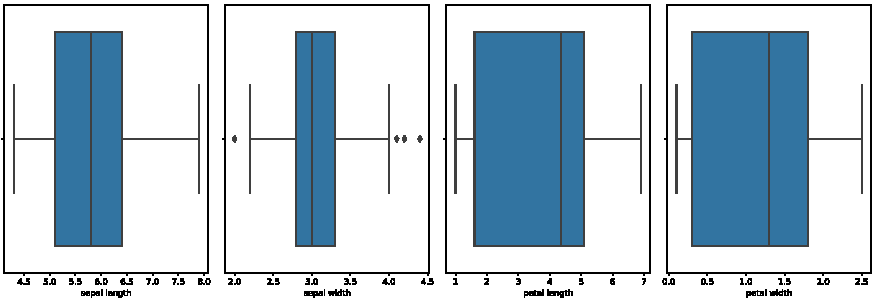
\includegraphics[width=\linewidth]{img/_iris_boxplot_general.pdf}
                \caption{Iris dataset general boxplot}
            \end{subfigure}%
            \begin{subfigure}{.5\textwidth}
                \centering
                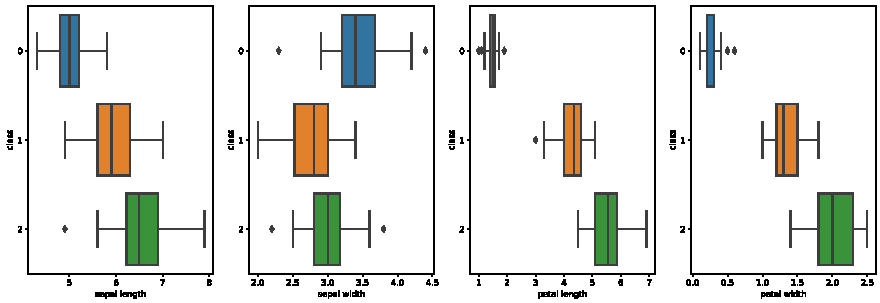
\includegraphics[width=\linewidth]{img/_iris_boxplot_inside.pdf}
                \caption{Iris dataset class boxplot}
            \end{subfigure}
            \begin{subfigure}{.5\textwidth}
                \centering
                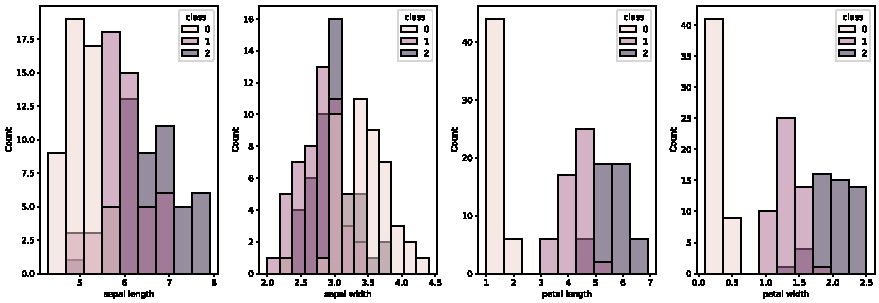
\includegraphics[width=\linewidth]{img/_iris_histogram.pdf}
                \caption{Iris dataset histograms}
            \end{subfigure}%
            \begin{subfigure}{.5\textwidth}
                \centering
                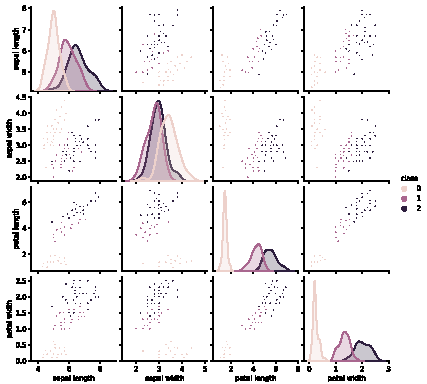
\includegraphics[width=\linewidth]{img/_iris_pairplot.pdf}
                \caption{Iris dataset pairplots}
            \end{subfigure}
        \end{figure}

    \item[Dataset split]
        A supervised dataset can be randomly split into:
        \begin{descriptionlist}
            \item[Train set] \marginnote{Train set}
                Used to learn the model. Usually the largest split.
            \item[Test set] \marginnote{Test set}
                Used to evaluate the trained model.
            \item[Validation set] \marginnote{Validation set}
                Used to evaluate the model during training.
        \end{descriptionlist}
        It is assumed that the splits have similar characteristics.

    \item[Overfitting] \marginnote{Overfitting}
        Given a dataset $\matr{X}$, a model $\mathcal{M}$ is overfitting if
        there exists another model $\mathcal{M}'$ such that:
        \[ 
            \begin{split}
                \texttt{error}_\text{train}(\mathcal{M}) &< \texttt{error}_\text{train}(\mathcal{M}') \\
                \texttt{error}_\matr{X}(\mathcal{M}) &> \texttt{error}_\matr{X}(\mathcal{M}') \\
            \end{split}    
        \]

        Possible causes of overfitting are:
        \begin{itemize}
            \item Noisy data.
            \item Lack of representative instances.
        \end{itemize}
\end{description}



\section{Decision trees}

\subsection{Information theory} \label{sec:information_theory}

\begin{description}
    \item[Shannon theorem] \marginnote{Shannon theorem}
        Let $\matr{X} = \{ \vec{v}_1, \dots, \vec{v}_V \}$ be a data source where 
        each of the possible value has probability $p_i = \prob{\vec{v}_i}$.
        The best encoding allows to transmit $\matr{X}$ with 
        an average number of bits given by the \textbf{entropy} of $X$: \marginnote{Entropy}
        \[ H(\matr{X}) = - \sum_j p_j \log_2(p_j) \]
        $H(\matr{X})$ can be seen as a weighted sum of the surprise factor $-\log_2(p_j)$.
        If $p_j \sim 1$, then the surprise of observing $\vec{v}_j$ is low, vice versa,
        if $p_j \sim 0$, the surprise of observing $\vec{v}_j$ is high.
        
        Therefore, when $H(\matr{X})$ is high, $\matr{X}$ is close to an uniform distribution.
        When $H(\matr{X})$ is low, $\matr{X}$ is close to a constant.

        \begin{example}[Binary source] \phantom{}\\
            \begin{minipage}{.50\linewidth}
                The two values of a binary source $\matr{X}$ have respectively probability $p$ and $(1-p)$.
                When $p \sim 0$ or $p \sim 1$, $H(\matr{X}) \sim 0$.\\
                When $p \sim 0.5$, $H(\matr{X}) \sim \log_2(2)=1$
            \end{minipage}
            \begin{minipage}{.45\linewidth}
                \centering
                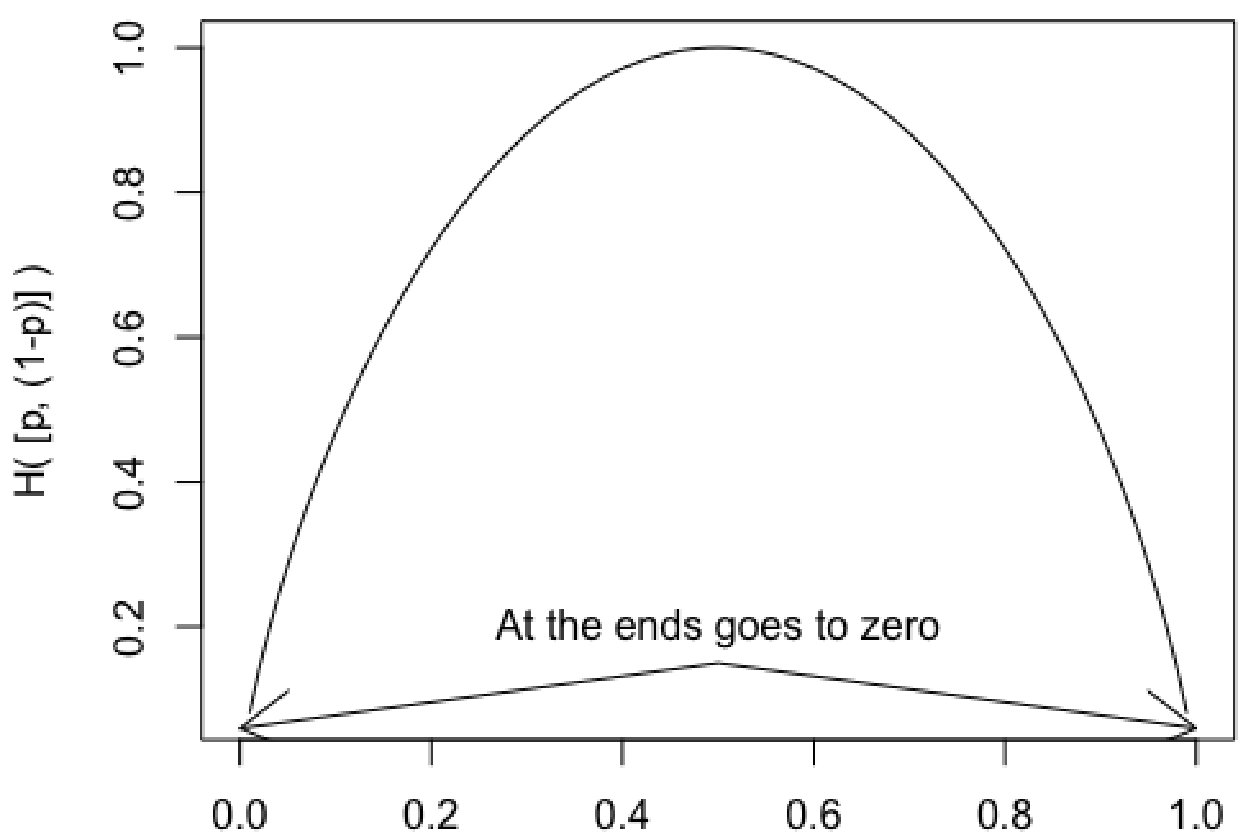
\includegraphics[width=\linewidth]{img/binary_entropy.png}
            \end{minipage}
        \end{example}

    \item[Entropy threshold split] \marginnote{Entropy threshold split}
        Given a dataset $\matr{D}$, 
        a real-valued attribute $d \in \matr{D}$,
        a threshold $t$ in the domain of $d$ and
        the class attribute $c$ of $\matr{D}$.
        The entropy of the class $c$ of the dataset $\matr{D}$ split with threshold $t$ on $d$ is a weighted sum:
        \[ H(c \,\vert\, d \,:\, t) = \prob{d < t}H(c \,\vert\, d < t) + \prob{d \geq t}H(c \,\vert\, d \geq t) \]

    \item[Information gain] \marginnote{Information gain}
        Information gain measures the reduction in entropy after applying a split.
        It is computed as:
        \[ IG(c \,\vert\, d \,:\, t) = H(c) - H(c \,\vert\, d \,:\, t) \]
        When $H(c \,\vert\, d \,:\, t)$ is low, $IG(c \,\vert\, d \,:\, t)$ is high 
        as splitting with threshold $t$ result in purer groups.
        Vice versa, when $H(c \,\vert\, d \,:\, t)$ is high, $IG(c \,\vert\, d \,:\, t)$ is low
        as splitting with threshold $t$ is not very useful.

        The information gain of a class $c$ split on a feature $d$ is given by:
        \[ IG(c \,\vert\, d) = \max_t IG(c \,\vert\, d \,:\, t) \]
\end{description}


\subsection{Tree construction}

\begin{description}
    \item[Decision tree (C4.5)] \marginnote{Decision tree}
        Tree-shaped classifier where leaves are class predictions and 
        inner nodes represent conditions that guide to a leaf.
        This type of classifier is non-linear (i.e. does not represent a linear separation).

        Each node of the tree contains:
        \begin{itemize}
            \item The applied splitting criteria (i.e. feature and threshold). 
                Leaves do not have this value.
            \item The entropy of the current split.
            \item Dataset coverage of the current split.
            \item Classes distribution.
        \end{itemize}

        \begin{figure}[h]
            \centering
            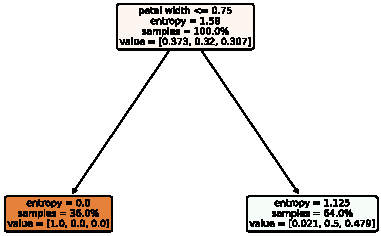
\includegraphics[width=0.5\textwidth]{img/_iris_decision_tree_example.pdf}
            \caption{Example of decision tree}
        \end{figure}

        Note: the weighted sum of the entropies of the children is always smaller than the entropy of the parent.

        Possible stopping conditions are:
        \begin{itemize}
            \item When most of the leaves are pure (i.e. nothing useful to split).
            \item When some leaves are impure but none of the possible splits have positive $IG$.
                Impure leaves are labeled with the majority class.
        \end{itemize}

    \item[Purity] \marginnote{Purity}
        Value to maximize when splitting a node of a decision tree.

        Nodes with uniformly distributed classes have a low purity.
        Nodes with a single class have the highest purity.

        Possible impurity measures are:
        \begin{descriptionlist}
            \item[Entropy/Information gain] See \Cref{sec:information_theory}. 

            \item[Gini index] \marginnote{Gini index}
                Let $\matr{X}$ be a dataset with classes $C$.
                The Gini index measures how often an element of $\matr{X}$ would be misclassified
                if the labels were randomly assigned based on the frequencies of the classes in $\matr{X}$.

                Given a class $i \in C$, $p_i$ is the probability (i.e. frequency) of classifying an element with $i$ and
                $(1 - p_i)$ is the probability of classifying it with a different label.
                The Gini index is given by:
                \[
                    \begin{split}
                        GINI(\matr{X}) = \sum_i^C p_i (1-p_i) &= \sum_i^C p_i - \sum_i^C p_i^2 \\
                            &= 1 - \sum_i^C p_i^2
                    \end{split}  
                \]
                When $\matr{X}$ is uniformly distributed, $GINI(\matr{X}) \sim (1-\frac{1}{\vert C \vert})$.
                When $\matr{X}$ is constant, $GINI(\matr{X}) \sim 0$.

                Given a node $p$ split in $n$ children $p_1, \dots, p_n$,
                the Gini gain of the split is given by:
                \[ GINI_\text{gain} = GINI(p) - \sum_{i=1}^n \frac{\vert p_i \vert}{\vert p \vert} GINI(p_i) \]
 
            \item[Misclassification error] \marginnote{Misclassification error}
                Skipped.
        \end{descriptionlist}

        \begin{figure}[h]
            \centering
            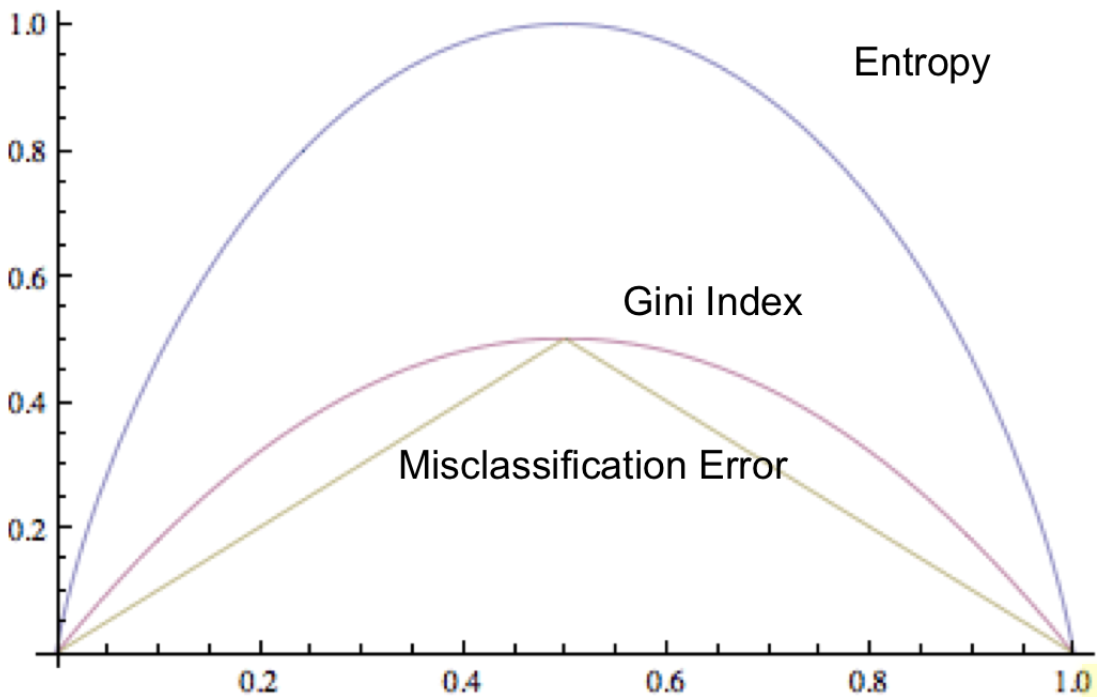
\includegraphics[width=0.35\textwidth]{img/impurity_comparison.png}
            \caption{Comparison of impurity measures}
        \end{figure}

        Compared to Gini index, entropy is more robust to noise.
\end{description}

\begin{algorithm}[H]
\caption{Decision tree construction using information gain as impurity measure}
\begin{lstlisting}
    def buildTree(split):
        node = Node()
        if len(split.classes) == 1: # Pure split
            node.label = split.classes[0]
            node.isLeaf = True
        else:
            ig, attribute, threshold = getMaxInformationGain(split)
            if ig < 0:
                node.label = split.majorityClass()
                node.isLeaf = True
            else:
                node.left = buildTree(split[attribute < threshold])
                node.right = buildTree(split[attribute >= threshold])
        return node
\end{lstlisting}
\end{algorithm}


\begin{description}
    \item[Pruning] \marginnote{Pruning}
        Remove branches to reduce overfitting.
\end{description}